\documentclass[11pt]{article}
\usepackage[T1]{fontenc}
\usepackage{lmodern,microtype}
\usepackage[a4paper,margin=28mm]{geometry}
\usepackage{amsmath,amssymb,amsthm,mathtools}
\usepackage{graphicx,booktabs,array,xcolor}
\usepackage[colorlinks=true,linkcolor=blue!45!black,citecolor=blue!45!black,urlcolor=blue!45!black]{hyperref}
\usepackage{enumitem}
\setlist{itemsep=3pt,topsep=5pt}
\newtheorem{theorem}{Theorem}[section]
\newtheorem{proposition}[theorem]{Proposition}
\newtheorem{lemma}[theorem]{Lemma}
\newtheorem{corollary}[theorem]{Corollary}
\theoremstyle{definition}
\newtheorem{definition}[theorem]{Definition}
\newtheorem{example}[theorem]{Example}
\theoremstyle{remark}
\newtheorem{remark}[theorem]{Remark}
\newcommand{\E}{\mathbb E}
\newcommand{\PP}{\mathbb P}
\newcommand{\1}{\mathbf 1}
\newcommand{\R}{\mathbb R}
\newcommand{\NN}{\mathbb N}
\newcommand{\shc}{\operatorname{sinhc}}
\DeclareMathOperator{\tr}{tr}
\DeclareMathOperator{\diag}{diag}
\title{Centered permutation products:\\ cancellation, the cubic threshold,\\ and critical asymptotics}
\author{}
\date{November 14, 2026}
\begin{document}
\maketitle
\begin{abstract}
We give a direct proof of the mixed centered permutation estimate used in random-lift and biregular spectral-gap arguments. Conditioning only on compatible prescribed matches produces a positive row-sum recurrence that keeps cancellation explicit. The bound allows arbitrary multiplicities and independent permutation colors, with the optimal universal prefactor $\sqrt e$ in the square-root range. For distinct centered diagonal entries, we prove that the leading terms of Collins and Nagatsu are relatively accurate exactly when $k^3/N\to0$, answering their published optimal-scale question. The critical even and odd limits are a hyperbolic cosine and a normalized hyperbolic sine. A positive partition expansion extends their relative accuracy to $k=o(\sqrt N)$. At $k^2/N\to d$, their missing correction is $e^{d/4}$, giving a uniformly accurate corrected formula on bounded square-root ranges. We explain the link to non-backtracking trace arguments and isolate two failures in an intermediate conditioning formula without challenging the underlying spectral theorem.
\end{abstract}
\tableofcontents
\clearpage
\section{The question and the proof mechanism}

A permutation matrix has one nonzero entry in every row and column. Its entries are therefore strongly dependent, even though each entry has mean $1/N$. This dependence has a useful consequence. Products of suitably separated centered entries are far smaller in expectation than one would predict by taking absolute values first.

For a uniform permutation matrix $M$ of size $N$, two distinct diagonal cells satisfy
\begin{equation}\label{eq:two}
\E\bigl[(M_{11}-N^{-1})(M_{22}-N^{-1})\bigr]
=\frac{1}{N(N-1)}-\frac{1}{N^2}
=\frac{1}{N^2(N-1)}.
\end{equation}
Two cells in the same row instead have centered product expectation $-N^{-2}$. The pattern of requested cells matters. The smaller scale in \eqref{eq:two} is cancellation, not independence.

The mixed-product estimate in Bordenave's Proposition 28 \cite{Bordenave} exploits this distinction. It also appears in Bordenave and Collins \cite[Proposition 22]{BC}. Brito, Dumitriu and Harris import it as Lemma 7 in their preprint, numbered Lemma 5.6 in the published article \cite{BDH}. We give a proof built from three operations:
\begin{enumerate}
\item Keep the isolated centered singletons together.
\item Condition only on a compatible set of prescribed matches. The remaining matrix is exactly a smaller uniform permutation matrix.
\item Use its row sum to obtain a positive recurrence, and only then expand the remaining factors.
\end{enumerate}
This order prevents the triangle inequality from destroying the cancellation we want to estimate.

For the diagonal product
\[
a_k(N)=\E\prod_{i=1}^k(M_{ii}-N^{-1}),
\]
Collins and Nagatsu establish the base recurrence, the parity-dependent leading terms, and the normalized error recurrences \cite[Proposition 3.3]{CN}. These are prior results. We reproduce their recurrence from a row-sum identity and use its positivity in the reverse direction, obtaining a lower bound that proves the cubic scale is necessary. A matching upper bound proves sufficiency. A continuous comparison then describes the transition itself.

\subsection{Main results at a glance}

Write $R_k=a_k/L_k$, where
\begin{equation}\label{eq:leading}
L_{2m}=(2m-1)!!N^{-3m},\qquad
L_{2m+1}=\frac{4m}{3}(2m+1)!!N^{-3m-2},\qquad m\ge1.
\end{equation}
The notation $(2m-1)!!$ means the product of the positive odd integers up to $2m-1$. The leading term for odd $k=1$ is zero, so $R_1$ is not defined.

We prove the following statements.
\begin{itemize}
\item For a mixed product involving $a$ distinct cells, with $h$ isolated centered singletons and $b$ nonisolated centered singletons,
\[
|\E P|\le\sqrt e\,2^b n^{-a}
\left(\frac{\sqrt{a-1}}{\sqrt n-\sqrt{a-1}}\right)^h,
\qquad 2\le a\le\sqrt n.
\]
Theorem~\ref{thm:mixed} includes arbitrary multiplicities, independent colors and a larger-range version.
\item For every $2\le k\le N$,
\[
R_k-1\ge\frac{2k^3}{27N}.
\]
If $2k\le N$, then $R_k\le\exp(3k^3/N)$. Hence $R_k\to1$ exactly when $k^3/N\to0$, and $R_k=O(1)$ exactly when $k^3/N=O(1)$.
\item If $k^3/N\to c<\infty$, the even and odd ratios tend respectively to
\[
\cosh\left(\frac23\sqrt c\right),\qquad
\shc\left(\frac23\sqrt c\right),
\]
where $\shc(z)=\sinh(z)/z$ for $z\ne0$ and $\shc(0)=1$. Theorem~\ref{thm:critical} gives a uniform finite-size error.
\item With $H_k$ equal to the corresponding hyperbolic approximation, $R_k/H_k\to1$ throughout $k=o(\sqrt N)$. If $k^2/N\to d>0$, then $R_k/H_k\to e^{d/4}$. Theorems~\ref{thm:window} and~\ref{thm:sqrt} give finite bounds and a uniform corrected approximation.
\end{itemize}

The mixed estimate supplies the requested probabilistic input to the graph arguments. The moment asymptotics answer a separate quantitative question about that input. They do not by themselves improve the final spectral-gap theorem.

\section{A direct mixed-product estimate}\label{sec:mixed}

Let $(\sigma_c)_c$ be independent uniform permutations of $[n]=\{1,\ldots,n\}$. Put $M_{cij}=\1_{\{\sigma_c(i)=j\}}$. A \emph{cell} is a triple $(c,i,j)$. Let $E$ be a nonempty finite set of distinct cells. Assign integers $p_e,q_e\ge0$ with $p_e+q_e\ge1$, and set
\begin{equation}\label{eq:product}
P=\prod_{e\in E}(M_e-n^{-1})^{p_e}M_e^{q_e},\qquad a=|E|.
\end{equation}
A cell is \emph{consistent} if no other cell of its color in $E$ shares its row or its column. A \emph{centered singleton} has $(p_e,q_e)=(1,0)$. Let $h$ and $b$ count the consistent and inconsistent centered singletons, respectively. Consistency is determined by the whole requested set, not by the realized permutation.

Write $(n)_r=n(n-1)\cdots(n-r+1)$ and $(n)_0=1$.

\begin{theorem}[Mixed centered products]\label{thm:mixed}
For $2\le a\le n$, define
\[
\beta=\frac{\sqrt{a-1}}{\sqrt n-\sqrt{a-1}},\qquad
F_n(q)=\frac{n^q}{(n)_q}\quad(0\le q\le n).
\]
Then
\begin{equation}\label{eq:mixedgeneral}
|\E P|\le F_n(a-h)\,2^b n^{-a}\beta^h
\le\exp\left(\frac{a(a-1)}{2(n-a+1)}\right)2^bn^{-a}\beta^h.
\end{equation}
If $a\le\sqrt n$, then
\begin{equation}\label{eq:mixedmain}
|\E P|\le\sqrt e\,2^b n^{-a}\beta^h
\le\sqrt e\,2^b n^{-a}\left(2\sqrt{a/n}\right)^h.
\end{equation}
For $a=1$, a centered singleton has expectation zero and every other product in \eqref{eq:product} has absolute expectation at most $1/n$.
\end{theorem}

The multiplicities in this statement have no upper bound. Increasing a repeated multiplicity does not incur an additional factor in the estimate. The constant $\sqrt e$ is optimal for this class of products, as shown at the end of the proof.

\subsection{Conditioning without losing the dimension}

Fix one color. A set of $r$ requested matches is \emph{compatible} if its rows and columns are all distinct. The event that all these matches occur has probability $1/(n)_r$. Given that event, delete their rows and columns. The remaining permutation is uniform on $N=n-r$ symbols.

Let $U$ denote its matrix and put $Z_{ij}=nU_{ij}-1$. We retain the original centering $1/n$, so every remaining row sums to $r$, not to zero. For $0\le j\le N$, let
\[
\mu_j(n,r)=\E\prod_{i=1}^j Z_{ii},\qquad \mu_0=1.
\]
By row and column symmetry, any $j$ remaining cells with distinct rows and columns have the same moment.

\begin{lemma}[Depleted row-sum recurrence]\label{lem:depleted}
For $1\le j\le n-r$,
\begin{equation}\label{eq:depleted}
(n-r-j+1)\mu_j=(r+2j-2)\mu_{j-1}+(j-1)\mu_{j-2},
\end{equation}
where the last term is omitted for $j=1$. In particular, every $\mu_j$ is nonnegative.
\end{lemma}
\begin{proof}
Multiply the last row sum, $\sum_{v=1}^{N}Z_{jv}=r$, by $Z_{11}\cdots Z_{j-1,j-1}$ and take expectations. There are $N-j+1$ columns unused by these factors. Each contributes $\mu_j$.

For a used column $i<j$, the indicator product $U_{ii}U_{ji}$ is zero. Hence
\[
Z_{ii}Z_{ji}=-Z_{ii}-Z_{ji}-1.
\]
After multiplying by the other $j-2$ diagonal factors, the two single-factor terms each have expectation $-\mu_{j-1}$. In the second term, interchange row labels $i$ and $j$ to see this. The last term contributes $-\mu_{j-2}$. Summing gives
\[
r\mu_{j-1}=(N-j+1)\mu_j-(j-1)(2\mu_{j-1}+\mu_{j-2}).
\]
This is \eqref{eq:depleted}. Its denominator is positive throughout the stated range, and its coefficients are nonnegative. Induction starts with $\mu_0=1$ and $\mu_1=r/(n-r)$.
\end{proof}

The case $r=0$, after rescaling, is the recurrence of Collins and Nagatsu \cite[Proposition 3.3, equation (16)]{CN}. The parameter $r$ records exactly how prescribed matches shift the remaining means.

\begin{lemma}[A geometric supersolution]\label{lem:super}
If $r+h\le a\le n$ and $a\ge2$, then $0\le\mu_h(n,r)\le\beta^h$.
\end{lemma}
\begin{proof}
The definition of $\beta$ gives the exact identity
\begin{equation}\label{eq:beta}
(n-a+1)\beta^2=2(a-1)\beta+(a-1).
\end{equation}
For $h\ge1$, we have $r\le a-1$ and
\[
\mu_1=\frac r{n-r}\le\frac{a-1}{n-a+1}\le\beta.
\]
For $2\le j\le h$, use
\[
r+2j-2\le2(a-1),\quad j-1\le a-1,\quad n-r-j+1\ge n-a+1.
\]
Substitute the induction bounds into \eqref{eq:depleted}, then use \eqref{eq:beta}. The case $h=0$ is immediate.
\end{proof}

\subsection{Only now expand the other factors}

Let $T$ be the consistent centered singletons. For each $e\notin T$, the indicator identity $M_e^2=M_e$ gives
\[
(M_e-n^{-1})^{p_e}M_e^{q_e}=c_e+d_eM_e.
\]
If $q_e\ge1$, then $c_e=0$ and $d_e=(1-1/n)^{p_e}\le1$. If $q_e=0$, then
\[
c_e=(-1/n)^{p_e},\qquad d_e=(1-1/n)^{p_e}-(-1/n)^{p_e}\ge0.
\]
The relevant coefficient weights obey
\begin{equation}\label{eq:weights}
d_e+n|c_e|\le
\begin{cases}
2,& (p_e,q_e)=(1,0),\\
1,& \text{otherwise}.
\end{cases}
\end{equation}
To check the only nontrivial case, put $x=1/n\le1/2$ and $p=p_e\ge2$. For even $p$,
\[
d_e+n|c_e|=(1-x)^p+(n-1)x^p
\le(1-x)^2+(n-1)x^2=1-x.
\]
For odd $p\ge3$,
\[
d_e+n|c_e|=(1-x)^p+(n+1)x^p
\le(1-x)^3+(n+1)x^3=1-3x+4x^2\le1-x.
\]
Thus a repeated centered cell costs at most one. Retaining this elementary inequality gives the prefactor $\sqrt e$ in \eqref{eq:mixedmain}.

Expand the affine factors, choosing a set $S\subseteq E\setminus T$ of prescribed indicators. Incompatible choices vanish. For a compatible choice, let $r_c$ and $h_c$ count its prescribed cells and the cells of $T$ in color $c$, respectively. The latter avoid every other requested row and column in that color. Therefore Lemma~\ref{lem:super} applies after conditioning, and
\begin{align}
\left|\E\prod_{e\in S}M_e\prod_{e\in T}(M_e-n^{-1})\right|
&\le n^{-h}\beta^h\prod_c\frac1{(n)_{r_c}}\notag\\
&=n^{-h-|S|}\beta^h\prod_c\frac{n^{r_c}}{(n)_{r_c}}.\label{eq:prescribed}
\end{align}
The factorial correction is bounded \emph{globally across colors}. For nonnegative $u,v$ with $u+v\le n$, the product definition gives $F_n(u)F_n(v)\le F_n(u+v)$. Since $\sum_c r_c=|S|\le a-h$, it follows that
\[
\prod_c F_n(r_c)\le F_n(|S|)\le F_n(a-h).
\]
For a simpler estimate, $-\log(1-x)\le x/(1-x)$ gives
\begin{align*}
\log\prod_c\frac{n^{r_c}}{(n)_{r_c}}
&\le\frac{\sum_c r_c(r_c-1)}{2(n-a+1)}\\
&\le\frac{a(a-1)}{2(n-a+1)}.
\end{align*}
This avoids multiplying an absolute constant once for every color.

Using \eqref{eq:prescribed} term by term in the affine expansion gives
\[
|\E P|\le F_n(a-h)n^{-a}\beta^h
\prod_{e\notin T}(d_e+n|c_e|)
\le F_n(a-h)2^bn^{-a}\beta^h.
\]
This proves \eqref{eq:mixedgeneral}. If $a^2\le n$, then $a(a-1)\le n-a+1$, so the exponential prefactor is at most $\sqrt e$. Also $\sqrt{(a-1)/n}\le1/2$, and hence $\beta\le2\sqrt{(a-1)/n}\le2\sqrt{a/n}$.

For $a=1$, the centered singleton has mean zero. If $q\ge1$, the absolute expectation is $n^{-1}(1-1/n)^p\le n^{-1}$. If $q=0$ and $p\ge2$, bound the absolute $p$th centered moment by the second, which is $n^{-1}(1-1/n)$. The case $n=1$ follows directly.

Finally, take $n=a^2$ and $P=M_{11}\cdots M_{aa}$ in one color. Then $h=b=0$ and $n^a\E P=F_n(a)$. As $a\to\infty$,
\[
\log F_{a^2}(a)=\sum_{j=0}^{a-1}-\log(1-j/a^2)
=\frac{a(a-1)}{2a^2}+O(a^{-1})\longrightarrow\frac12.
\]
No smaller universal prefactor can replace $\sqrt e$ in \eqref{eq:mixedmain} for all the permitted products.

\subsection{A conditional example}

For $n\ge3$, prescribe $M_{11}=1$ and retain two disjoint centered cells. Lemma~\ref{lem:depleted} with $r=1$ gives
\[
\mu_1=\frac1{n-1},\qquad
\mu_2=\frac{n+2}{(n-1)(n-2)}.
\]
Consequently,
\[
\E\bigl[M_{11}(M_{22}-n^{-1})(M_{33}-n^{-1})\bigr]
=\frac{n+2}{n^3(n-1)(n-2)}.
\]
The remaining centered entries do not have conditional mean zero. Their mean shift is already built into the recurrence.

\section{The exact cubic threshold}\label{sec:threshold}

We now study $a_k(N)$ and $R_k=a_k/L_k$ from \eqref{eq:leading}, always with $2\le k\le N$. The matrix size is denoted by $N$ to distinguish this analysis from the depleted permutation in Section~\ref{sec:mixed}.

\begin{theorem}[Necessary and sufficient scale]\label{thm:threshold}
For every $2\le k\le N$,
\begin{equation}\label{eq:lower}
R_k-1\ge\frac{2k^3}{27N}.
\end{equation}
For $2k\le N$,
\begin{equation}\label{eq:upper}
R_k\le\exp(3k^3/N).
\end{equation}
Consequently, for every integer sequence $2\le k_N\le N$ as $N\to\infty$,
\begin{align}
R_{k_N}\to1&\quad\Longleftrightarrow\quad k_N^3/N\to0,\label{eq:iff}\\
R_{k_N}=O(1)&\quad\Longleftrightarrow\quad k_N^3/N=O(1).\label{eq:bounded}
\end{align}
The lower-bound constant $2/27$ is optimal uniformly over both parities.
\end{theorem}

The necessity in this result addresses the question in Collins and Nagatsu's published Remark 3.4 \cite{CN}. The statement concerns relative accuracy of their specific leading terms. It does not say that centered products cease to have useful upper bounds outside the cubic range.

\subsection{The known recurrence and its normalization}

Lemma~\ref{lem:depleted} with $r=0$, after rescaling, gives
\begin{equation}\label{eq:momentrec}
a_k=\frac{2(k-1)}{N(N-k+1)}a_{k-1}
+\frac{k-1}{N^2(N-k+1)}a_{k-2},
\qquad a_0=1,\quad a_1=0.
\end{equation}
This is \cite[equation (16)]{CN}. Its coefficients show that $a_k>0$ for $2\le k\le N$.

Set $E_k=R_k-1$. Substitution of \eqref{eq:leading} into \eqref{eq:momentrec} gives the following normalized recurrences, also present in the proof of \cite[Proposition 3.3]{CN}. For $m\ge2$,
\begin{align}
E_{2m}={}&\frac{N}{N-2m+1}E_{2m-2}
+\frac{4(2m-1)(2m-2)}{3(N-2m+1)}E_{2m-1}\notag\\
&+\frac{(2m-1)(8m-5)}{3(N-2m+1)}.\label{eq:evenerror}
\end{align}
For $m\ge1$,
\begin{align}
E_{2m+1}={}&\frac{3N}{(N-2m)(2m+1)}E_{2m}
+\frac{(2m-2)N}{(N-2m)(2m+1)}E_{2m-1}
+\frac{2m}{N-2m},\label{eq:odderror}
\end{align}
where the term involving $E_1$ is omitted at $m=1$. The initial error is $E_2=1/(N-1)$. Every coefficient and forcing term is nonnegative. In particular, $E_k\ge0$.

\subsection{Accumulating a lower bound}

In \eqref{eq:evenerror}, discard the second nonnegative term and bound the other denominator by $N$. This gives
\[
E_{2m}\ge E_{2m-2}+\frac{(2m-1)(8m-5)}{3N}.
\]
At $m=1$, the same inequality means $E_2\ge1/N$, with $E_0=0$ used only for the summation. Summing yields
\begin{equation}\label{eq:evenlower}
E_{2m}\ge\frac{C_{\rm e}(m)}N,
\qquad C_{\rm e}(m)=\frac{m(16m^2-3m-4)}9.
\end{equation}
The right side is at least $m^3/N$, because
\[
C_{\rm e}(m)-m^3=\frac{m(m-1)(7m+4)}9\ge0.
\]

For the odd orders define
\[
C_{\rm o}(m)=\frac{80m^3+195m^2+124m+6}{135}.
\]
A direct polynomial calculation gives $C_{\rm o}(1)=3$ and
\begin{equation}\label{eq:oddpoly}
C_{\rm o}(m)=\frac{3C_{\rm e}(m)+(2m-2)C_{\rm o}(m-1)}{2m+1}+2m.
\end{equation}
Equation~\eqref{eq:odderror} implies
\[
E_{2m+1}\ge\frac{3E_{2m}+(2m-2)E_{2m-1}}{2m+1}+\frac{2m}N.
\]
Induction using \eqref{eq:evenlower} and \eqref{eq:oddpoly} proves
\begin{equation}\label{eq:oddlower}
E_{2m+1}\ge C_{\rm o}(m)/N.
\end{equation}
At $m=1$, this starts from $E_3\ge E_2+2/N\ge3/N$. Finally,
\[
C_{\rm o}(m)-\frac{2(2m+1)^3}{27}
=\frac{75m^2+64m-4}{135}>0.
\]
For the even orders, $m^3\ge2(2m)^3/27$. Together these inequalities prove \eqref{eq:lower}.

\subsection{A self-contained upper bound}

Suppose $2k\le N$. In the recurrences for $R_j$, obtained by adding one back to \eqref{eq:evenerror} and \eqref{eq:odderror}, the sum of the coefficients is
\[
1+\frac{(2m-1)(8m-5)}{3(N-2m+1)}
\quad\text{for }j=2m,
\]
and $N/(N-2m)$ for $j=2m+1$. In both cases it is at most $1+3j^2/N$, using $N-j+1\ge N/2$. The same bound starts the induction at $R_2=N/(N-1)$. Positivity gives
\[
\max(1,R_2,\ldots,R_k)
\le\prod_{j=2}^k(1+3j^2/N)
\le\exp\left(\frac3N\sum_{j=2}^k j^2\right)
\le\exp(3k^3/N).
\]
This proves \eqref{eq:upper}.

If $k_N^3/N\to0$ or merely stays bounded, then $2k_N\le N$ eventually. The two bounds now imply \eqref{eq:iff} and \eqref{eq:bounded}. Sharpness of $2/27$ follows from Corollary~\ref{cor:small} below.

\begin{example}[Order four]
The recurrence gives
\[
a_4(N)=\frac{3(N+6)}{N^4(N-1)(N-2)(N-3)},\qquad
R_4(N)=\frac{N^2(N+6)}{(N-1)(N-2)(N-3)}.
\]
Thus $R_4=1+12/N+O(N^{-2})$. A fixed-order expansion like this is useful for checking normalization. The threshold theorem needs the uniform argument above, because its order is allowed to grow with $N$.
\end{example}

\section{The critical transition and its parity}\label{sec:critical}

The cubic threshold is visible in the normalized recurrence: the even ratio changes by order $m^2/N$ at step $m$, and summing this over $m$ steps produces $m^3/N$. At the transition, these increments cannot be discarded. They converge to a coupled differential system.

\begin{theorem}[Uniform critical approximation]\label{thm:critical}
For every fixed $T>0$ there is a finite $C_T$ such that, whenever $M\ge1$, $N\ge4M+2$ and $M^3/N\le T$,
\begin{align}
\max_{1\le m\le M}\left|R_{2m}-\cosh z_m\right|&\le C_T M^2/N,\label{eq:criticeven}\\
\max_{1\le m\le M}\left|R_{2m+1}-\shc z_m\right|&\le C_T M^2/N,\label{eq:criticodd}
\end{align}
where $z_m=(4\sqrt2/3)\sqrt{m^3/N}$. If $k_N^3/N\to c\in[0,\infty)$, then
\begin{align*}
R_{k_N}&\longrightarrow\cosh\left(\frac23\sqrt c\right)
&&\text{along even orders},\\
R_{k_N}&\longrightarrow\shc\left(\frac23\sqrt c\right)
&&\text{along odd orders at least three}.
\end{align*}
For $c>0$, the two limits are different.
\end{theorem}

\subsection{The exact two-component recursion}

Put $e_m=R_{2m}$ and $o_m=R_{2m+1}$ for $m\ge1$, with auxiliary seeds $e_0=o_0=1$. These seeds do not define $R_0$ or $R_1$. The coefficients multiplying $o_0$ vanish at the first step. Equation~\eqref{eq:momentrec} gives
\begin{equation}\label{eq:tworec}
e_m=A_me_{m-1}+B_mo_{m-1},\qquad
o_m=C_me_m+D_mo_{m-1},
\end{equation}
where
\begin{align*}
A_m&=\frac N{N-2m+1},&
B_m&=\frac{4(2m-1)(2m-2)}{3(N-2m+1)},\\
C_m&=\frac{3N}{(N-2m)(2m+1)},&
D_m&=\frac{(2m-2)N}{(N-2m)(2m+1)}.
\end{align*}
At $m=1$, these reproduce $R_2=N/(N-1)$ and $R_3=N^2/((N-1)(N-2))$. Under $N\ge4M+2$, all coefficients are nonnegative and
\begin{equation}\label{eq:rowsums}
A_m+B_m\le1+12m^2/N,\qquad
C_m+D_m\le1+4m^2/N,\qquad C_m\le2.
\end{equation}
For example, the first row sum has excess
\[
\frac{(2m-1)(8m-5)}{3(N-2m+1)}\le\frac{32m^2}{3N}.
\]
The second row sum is $N/(N-2m)$, with excess at most $4m/N$.

\subsection{A comparison system with an explicit solution}

For $x\ge0$ set
\[
z(x)=\frac{4\sqrt2}{3}\sqrt{x^3/N},\qquad
E(x)=\cosh z(x),\qquad O(x)=\shc z(x).
\]
Direct differentiation gives
\begin{equation}\label{eq:ode}
E'(x)=\frac{16x^2}{3N}O(x),\qquad
O'(x)=\frac3{2x}(E(x)-O(x)).
\end{equation}
The second identity extends continuously to $x=0$. The associated power series are
\[
E(x)=\sum_{\ell\ge0}\frac{(32x^3/(9N))^\ell}{(2\ell)!},\qquad
O(x)=\sum_{\ell\ge0}\frac{(32x^3/(9N))^\ell}{(2\ell+1)!}.
\]
For $x^3/N\le T$, termwise differentiation therefore gives
\begin{align}
|E(x)|+|O(x)|&\le K_T,&
|E(x)-O(x)|&\le K_Tx^3/N,\notag\\
|E'(x)|+|O'(x)|&\le K_Tx^2/N,&
|E''(x)|+|O''(x)|&\le K_Tx/N.\label{eq:derivatives}
\end{align}
The derivative estimates follow by factoring $x^2/N$ or $x/N$ from the differentiated series. The remaining series converge uniformly on the bounded interval for $x^3/N$.

\subsection{Local errors and stability}

Write $E_m=E(m)$ and $O_m=O(m)$. The residuals of \eqref{eq:tworec} are
\[
\rho_m^E=E_m-A_mE_{m-1}-B_mO_{m-1},\qquad
\rho_m^O=O_m-C_mE_m-D_mO_{m-1}.
\]
We claim that
\begin{equation}\label{eq:residual}
|\rho_m^E|+|\rho_m^O|\le K'_Tm/N.
\end{equation}
Taylor's theorem and \eqref{eq:derivatives} bound each backward difference minus its derivative at $m$ by $O_T(m/N)$. With $b_m=16m^2/(3N)$, the exact coefficients give
\[
A_m-1=O(m/N),\qquad B_m-b_m=O_T(m/N).
\]
For the second estimate, direct subtraction bounds the difference by a constant times $m/N+m^3/N^2$, which is $O_T(m/N)$. Now
\begin{align*}
\rho_m^E={}&E_m-E_{m-1}-E'(m)+b_m(O_m-O_{m-1})\\
&-(A_m-1)E_{m-1}-(B_m-b_m)O_{m-1}.
\end{align*}
Every term is $O_T(m/N)$. In particular, the second term is $O_T(m^4/N^2)$, and $m^3/N\le T$ makes it $O_T(m/N)$.

For the odd residual write
\[
c_m=\frac3{2m+1},\quad d_m=\frac{2m-2}{2m+1},\quad t_m=\frac N{N-2m}.
\]
Then $c_m+d_m=1$, $C_m=t_mc_m$, $D_m=t_md_m$ and $t_m-1=O(m/N)$. Removing $t_m$ changes the residual by $O_T(m/N)$. The remaining expression is
\[
d_m(O_m-O_{m-1})-c_m(E_m-O_m).
\]
After substituting \eqref{eq:ode}, the coefficient of $E_m-O_m$ is
\[
d_m\frac3{2m}-c_m=-\frac3{m(2m+1)}.
\]
Equation~\eqref{eq:derivatives} bounds its contribution by $O_T(m/N)$, proving \eqref{eq:residual}, including at $m=1$.

Let $H_m=\max(|e_m-E_m|,|o_m-O_m|)$ and $H_0=0$. Subtract the comparison equations from \eqref{eq:tworec}. First bound the even error, then use that bound in the odd equation. Positivity and \eqref{eq:rowsums} yield
\[
H_m\le(1+12m^2/N)(1+4m^2/N)H_{m-1}+3K'_Tm/N.
\]
The product of all multiplicative factors through step $M$ is at most
\[
\exp\left(\frac{16}N\sum_{m=1}^M m^2\right)\le e^{16T}.
\]
Summing the local errors proves $\max_{m\le M}H_m\le3K'_Te^{16T}M^2/N$, establishing \eqref{eq:criticeven} and \eqref{eq:criticodd}.

If $k^3/N$ stays bounded, then $m=O(N^{1/3})$ and the error tends to zero. For even $k=2m$, $z_m^2=4k^3/(9N)$. For odd $k=2m+1$, replacing $(2m)^3/N$ by $k^3/N$ changes it by $O(m^2/N)$. Continuity proves the stated limits.

\begin{corollary}[Small relative errors and sharpness]\label{cor:small}
If $k\to\infty$ and $k^3/N\to0$, then
\[
R_k-1\sim\frac{2k^3}{9N}\quad\text{for even }k,
\qquad
R_k-1\sim\frac{2k^3}{27N}\quad\text{for odd }k.
\]
Thus the constant $2/27$ in Theorem~\ref{thm:threshold} cannot be increased.
\end{corollary}
\begin{proof}
Take a fixed $T$, for instance $T=1$. The error $O(M^2/N)$ with $M$ equal to the relevant $m$ is smaller than $k^3/N$ by a factor of order $1/k$. Expand $\cosh z=1+z^2/2+O(z^4)$ and $\shc z=1+z^2/6+O(z^4)$.
\end{proof}

\begin{example}[A transition visible without a large formula]
When $k^3/N\to9/4$, the two limits are $\cosh(1)\approx1.5431$ and $\sinh(1)\approx1.1752$. Both exceed one. Their difference shows why an arbitrary sequence containing both parities need not have a common normalized limit.
\end{example}

\section{Positive partitions and a wider asymptotic window}\label{sec:extension}

The recurrence admits a positive coefficient representation. It explains the hyperbolic functions by counting pairs and triples, and extends their relative accuracy well beyond the critical cubic range. At the square-root scale, a further correction becomes visible.

For $k\ge2$, put $m=\lfloor k/2\rfloor$, $K=2m$ and
\begin{equation}\label{eq:hyperdef}
\lambda=\frac23\sqrt{K^3/N},\qquad
H_k=\begin{cases}\cosh\lambda,&k\text{ even},\\
\shc\lambda,&k\text{ odd}.
\end{cases}
\end{equation}
For odd $k$, the definition intentionally uses $K=k-1$.

\begin{figure}[tbp]
\centering
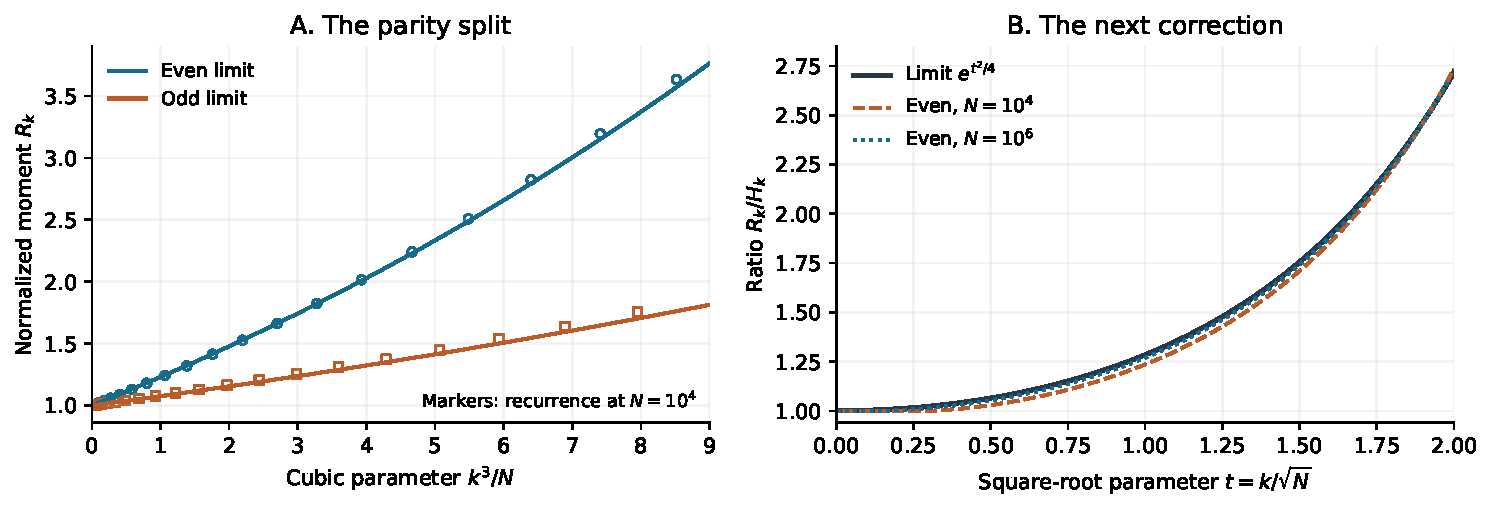
\includegraphics[width=\textwidth]{../figures/moment-regimes.pdf}
\caption{The two transitions. Left: the parity-dependent critical limits and recurrence evaluations at $N=10^4$. Right: the ratio to the hyperbolic approximation at even orders, compared with its square-root correction. Curves illustrate the proved statements and are not premises of the proofs.}
\label{fig:regimes}
\end{figure}

\begin{theorem}[Relative hyperbolic approximation]\label{thm:window}
For integers $2\le k\le N/4$,
\begin{equation}\label{eq:envelope}
\left(1-\frac{4k^2}{3N}\right)H_k
\le R_k\le e^{4k^2/N}H_k.
\end{equation}
If $4k^2\le N$, then
\begin{equation}\label{eq:logerror}
-\frac{2k^2}N\le\log\frac{R_k}{H_k}\le\frac{4k^2}N.
\end{equation}
Consequently $R_k/H_k\to1$ whenever $k=o(\sqrt N)$, even if $k^3/N\to\infty$.
\end{theorem}

\begin{theorem}[The square-root correction]\label{thm:sqrt}
If $k^2/N\to d\in(0,\infty)$, then
\begin{equation}\label{eq:sqrtlimit}
\frac{R_k}{H_k}\longrightarrow e^{d/4}.
\end{equation}
For every fixed $C>0$,
\begin{equation}\label{eq:uniformsqrt}
\sup_{2\le k\le C\sqrt N}
\left|\frac{R_k}{e^{k^2/(4N)}H_k}-1\right|\longrightarrow0,
\end{equation}
where the supremum is over integers and $N\to\infty$.
\end{theorem}

Thus the uncorrected hyperbolic approximation loses relative accuracy at every positive square-root scale. The corrected expression is uniformly accurate on bounded multiples of that scale. We assert neither a rate in \eqref{eq:uniformsqrt} nor an approximation for unbounded $k/\sqrt N$.

\subsection{Clearing the denominators}

Set $Q_k=(N)_kN^ka_k$, with $Q_0=1$ and $Q_1=0$. Equation~\eqref{eq:momentrec} becomes
\begin{equation}\label{eq:qrec}
Q_k=2(k-1)Q_{k-1}+(k-1)(N-k+2)Q_{k-2}.
\end{equation}
Extend this polynomial recurrence formally to all orders. This algebraic extension does not define permutation moments for $k>N$. The exponential generating function $F(z)=\sum_{k\ge0}Q_kz^k/k!$ satisfies
\[
(1-z)^2F'(z)=NzF(z),\qquad F(0)=1.
\]
Consequently,
\begin{equation}\label{eq:egf}
F(z)=\exp\left(N\left[\frac z{1-z}+\log(1-z)\right]\right)
=\exp\left(N\sum_{j\ge2}\frac{j-1}{j}z^j\right).
\end{equation}
This is a classical Laguerre generating function: $Q_k=k!L_k^{(-N-1)}(-N)$ \cite[equations 18.5.12 and 18.12.13]{DLMF}. It is also a reformulation of the special-function identification in \cite[Remark 3.5]{CN}. We derive it here to use its positive coefficients, not as a new special-function identity.

Extracting coefficients gives
\begin{equation}\label{eq:partitions}
Q_k=k!\sum_{\substack{c_2,c_3,\ldots\ge0\\\sum_{j\ge2}jc_j=k}}
\prod_{j\ge2}\frac{(N(j-1)/j)^{c_j}}{c_j!}.
\end{equation}
Equivalently, this is a weighted count of labeled set partitions without singleton blocks. A block of size $j$ has weight $N(j-1)(j-1)!$. Pairs have weight $N$, and triples have weight $4N$.

Define the polynomial leading terms
\[
\mathcal L_{2m}=(2m-1)!!N^m,\qquad
\mathcal L_{2m+1}=\frac{4m}{3}(2m+1)!!N^m.
\]
They count all-pair partitions and one-triple partitions, respectively. Indeed, the latter coefficient is
\[
\binom{2m+1}{3}4(2m-3)!!=\frac{4m}{3}(2m+1)!!.
\]
With $D_k=N^k/(N)_k$, the normalization is exactly
\begin{equation}\label{eq:qnormalize}
R_k=D_k\frac{Q_k}{\mathcal L_k}.
\end{equation}

\subsection{The number of available pairs}

For blocks of size at least three put
\[
S=\sum_{j\ge3}jc_j,\qquad x=\sqrt{K/N},\qquad
\lambda_j=N\frac{j-1}{j}x^j.
\]
In particular, $\lambda_3=\lambda$. Cancelling the pair factorial in \eqref{eq:partitions} against the one in $\mathcal L_k$, the normalized contribution of these nonpair counts is
\begin{equation}\label{eq:availabilityeven}
\frac{(m)_{S/2}}{m^{S/2}}
\prod_{j\ge3}\frac{\lambda_j^{c_j}}{c_j!}
\quad\text{if }k=2m\text{ and }S\text{ is even},
\end{equation}
and
\begin{equation}\label{eq:availabilityodd}
\frac{(m-1)_{(S-3)/2}}{m^{(S-3)/2}}
\frac1\lambda\prod_{j\ge3}\frac{\lambda_j^{c_j}}{c_j!}
\quad\text{if }k=2m+1\text{ and }S\text{ is odd}.
\end{equation}
An odd $S$ here is at least three. A falling factorial with too many factors is assigned zero. The availability factors lie in $[0,1]$ and enforce the requirement that enough pairs remain.

\subsection{Proof of the finite relative bounds}

Assume $k\le N/4$, so $x\le1/2$. Put
\[
A_* =\sum_{\substack{j\ge4\\j\text{ even}}}\lambda_j,
\qquad B_* =\sum_{\substack{j\ge3\\j\text{ odd}}}\lambda_j.
\]
Remove the availability factors and project the exponential series onto the required parity. This gives
\[
\frac{Q_{2m}}{\mathcal L_{2m}}\le e^{A_*}\cosh B_*,\qquad
\frac{Q_{2m+1}}{\mathcal L_{2m+1}}\le e^{A_*}\frac{\sinh B_*}{\lambda}.
\]
The extra block weights satisfy
\begin{align*}
A_*+B_*-\lambda&\le\frac{Nx^4}{1-x}\le\frac{2K^2}N,\\
\frac{B_*}{\lambda}&\le1+\frac{3x^2}{2(1-x^2)}
\le1+\frac{2K}N\le e^{K^2/N}.
\end{align*}
The logarithmic derivatives of $\cosh t$ and $\shc t$ lie in $[0,1]$ for $t>0$. For the latter this follows from $0\le\coth t-1/t\le1$. Thus
\[
Q_k/\mathcal L_k\le e^{3K^2/N}H_k.
\]
Also
\[
\log D_k\le\frac{k(k-1)}{2(N-k+1)}\le k^2/N.
\]
Equation~\eqref{eq:qnormalize} proves the upper bound in \eqref{eq:envelope}.

For the lower bound, retain only pairs and triples. At even order, with $J$ triples,
\[
\frac{Q_{2m}}{\mathcal L_{2m}}
\ge\sum_{\ell\ge0}\frac{\lambda^{2\ell}}{(2\ell)!}
\frac{(m)_{3\ell}}{m^{3\ell}}.
\]
For any integer $s\ge0$,
\[
\frac{(m)_s}{m^s}\ge1-\frac{s(s-1)}{2m}.
\]
This follows from the product bound $\prod_i(1-u_i)\ge1-\sum_i u_i$ for $0\le u_i\le1$. If $s>m$, the left side is zero and the right side is nonpositive.

Normalize $\lambda^J/J!$ on even $J$ by $\cosh\lambda$. Then
\[
\E J=\lambda\tanh\lambda,\qquad
\E J^2=\lambda^2+\lambda\tanh\lambda.
\]
With $s=3J/2$, the relative loss is at most
\[
\frac{9\lambda^2+3\lambda\tanh\lambda}{8m}
\le\frac{3\lambda^2}{2m}=\frac{4K^2}{3N}.
\]
For odd order the analogous series is
\[
\frac{Q_{2m+1}}{\mathcal L_{2m+1}}
\ge\sum_{\ell\ge0}\frac{\lambda^{2\ell}}{(2\ell+1)!}
\frac{(m-1)_{3\ell}}{m^{3\ell}}.
\]
Now $(m-1)_s/m^s\ge1-s(s+1)/(2m)$. Normalize $\lambda^J/J!$ on odd $J$ by $\sinh\lambda$ and use $s=3(J-1)/2$. The relative loss is at most
\[
\frac{9\lambda^2-3\lambda\coth\lambda+3}{8m}
\le\frac{9\lambda^2}{8m}=\frac{K^2}N,
\]
because $\lambda\coth\lambda\ge1$. Multiplying by $D_k\ge1$ proves the lower half of \eqref{eq:envelope}. If its factor is negative, positivity suffices. Finally, $\log(1-4u/3)\ge-2u$ for $0\le u\le1/4$, proving \eqref{eq:logerror} and Theorem~\ref{thm:window}.

\subsection{Proof of the square-root correction}

Suppose $k^2/N\to d\in(0,\infty)$. Let $C_j$, $j\ge3$, be independent Poisson variables with means $\lambda_j$, and put
\[
\Lambda=\sum_{j\ge3}\lambda_j,\qquad S=\sum_{j\ge3}jC_j.
\]
For all sufficiently large $N$, $x<1$, so the total mean is finite and only finitely many $C_j$ are nonzero almost surely. Define
\[
w_{\rm e}(s)=(m)_s/m^s\quad(0\le s\le m),\qquad
w_{\rm o}(s)=(m-1)_s/m^s\quad(0\le s\le m-1),
\]
with value zero outside the respective integer ranges. The exact sums \eqref{eq:availabilityeven} and \eqref{eq:availabilityodd} become
\begin{align}
\frac{Q_{2m}}{\mathcal L_{2m}}
&=e^\Lambda\E\bigl[\1_{\{S\text{ even}\}}w_{\rm e}(S/2)\bigr],\label{eq:poissoneven}\\
\frac{Q_{2m+1}}{\mathcal L_{2m+1}}
&=\frac{e^\Lambda}{\lambda}\E\bigl[\1_{\{S\text{ odd}\}}w_{\rm o}((S-3)/2)\bigr].\label{eq:poissonodd}
\end{align}
Each availability function is evaluated only on its displayed parity event.

First control all block sizes:
\[
\lambda\to\infty,\qquad
\lambda_4=\frac{3K^2}{4N}\to\frac{3d}4,\qquad
\sum_{j\ge5}\lambda_j\le\frac{Nx^5}{1-x}\to0.
\]
Therefore $C_3/\lambda\to1$ in probability, $C_4=O_{\PP}(1)$, and the probability of any larger block tends to zero. Also $\Lambda-\lambda\to3d/4$.

On the event of no larger block, the argument $s$ of either availability function is $3C_3/2+2C_4+O(1)$. Since $\lambda^2/m\to8d/9$, we obtain, on the relevant parity event,
\[
\frac{s^2}{2m}\to d,\qquad \frac sm\to0,\qquad \frac{s^3}{m^2}\to0
\]
in probability. For $s/m\le1/2$, expansion of the logarithm gives
\[
\log w_{\rm e}(s)=-\frac{s(s-1)}{2m}+O(s^3/m^2),\qquad
\log w_{\rm o}(s)=-\frac{s(s+1)}{2m}+O(s^3/m^2).
\]
For example, these follow by summing
$0\le-\log(1-u)-u\le u^2/(2(1-u))$.
Thus each availability factor approaches $e^{-d}$ on its relevant parity event. All factors lie in $[0,1]$, so the corresponding error multiplied by the parity indicator tends to zero in mean.

The Poisson parity identity gives
\[
\PP(S\text{ even})=\frac{1+e^{-2B_*}}2,\qquad
\PP(S\text{ odd})=\frac{1-e^{-2B_*}}2.
\]
Because $B_*\ge\lambda\to\infty$, both probabilities tend to $1/2$. Hence both expectations in \eqref{eq:poissoneven} and \eqref{eq:poissonodd} tend to $e^{-d}/2$. No independence between parity and availability is required.

Since $\cosh\lambda\sim e^\lambda/2$ and $\sinh\lambda\sim e^\lambda/2$,
\[
\frac{Q_k/\mathcal L_k}{H_k}\longrightarrow e^{3d/4-d}=e^{-d/4}.
\]
Finally,
\[
\log D_k=\frac{k(k-1)}{2N}+O(k^3/N^2)\longrightarrow d/2.
\]
Restoring $D_k$ in \eqref{eq:qnormalize} proves \eqref{eq:sqrtlimit}. The three contributions are $3d/4$ from four-blocks, $-d$ from pair depletion and $d/2$ from the permutation probability.

To prove \eqref{eq:uniformsqrt}, suppose its supremum failed to tend to zero. Select a sequence of offending orders and pass to a subsequence on which $k^2/N\to d\in[0,C^2]$. If $d=0$, Theorem~\ref{thm:window} gives convergence to one. If $d>0$, \eqref{eq:sqrtlimit} gives it. Both contradict the selection.

\subsection{A worked partition count}

The first polynomials include
\[
Q_2=N,\quad Q_3=4N,\quad Q_4=3N^2+18N,\quad
Q_6=15N^3+430N^2+600N.
\]
For $Q_6$, the four contributions are
\begin{center}
\begin{tabular}{lr}
\toprule
Block sizes & Contribution\\
\midrule
$2+2+2$ & $15N^3$\\
$3+3$ & $160N^2$\\
$2+4$ & $270N^2$\\
$6$ & $600N$\\
\bottomrule
\end{tabular}
\end{center}
At the cubic scale, triples have bounded effective weight, while four-blocks and pair depletion disappear. Summing an even or odd number of triples gives the two hyperbolic functions. At the square-root scale, the four-block weight and pair depletion survive, producing the correction in Theorem~\ref{thm:sqrt}.

In the intermediate regime $N^{1/3}\ll k\ll\sqrt N$, Theorem~\ref{thm:window} also yields
\[
R_k\sim\tfrac12e^\lambda\quad(k\text{ even}),\qquad
R_k\sim\frac{e^\lambda}{2\lambda}\quad(k\text{ odd}).
\]
At $k\sim\sqrt N$, the ratio to the uncorrected hyperbolic term tends instead to $e^{1/4}\approx1.2840$.

\section{Where the estimate enters spectral-gap arguments}\label{sec:spectral}

This section identifies the application of Theorem~\ref{thm:mixed} and explains the surrounding mechanism. The graph-level path enumeration and tangle estimates are separate ingredients from the papers cited below.

\subsection{Random lifts: one permutation per base edge}

In Bordenave's model, choose one orientation of each undirected edge of a finite base graph. Attach an independent uniform permutation of $[n]$ to each chosen edge. Its reverse orientation carries the inverse permutation. A lift edge between fibers is represented by a matrix entry of this permutation, and reversing the edge transposes the same entry.

Orient every factor in a requested product according to the chosen base orientations. Base edges become colors in \eqref{eq:product}. Distinct requested lift edges become distinct cells. Their multiplicities and consistency conditions are unchanged. The parameter $a_1$ of \cite[Proposition 28]{Bordenave} is exactly $h$ here, and its inconsistent centered-singleton count is $b$.

If the original product has $k$ factors, then $a\le k\le\sqrt n$. For $a\ge2$, Theorem~\ref{thm:mixed} gives
\[
|\E P|\le\sqrt e\,2^bn^{-a}(2\sqrt{a/n})^{a_1}
\le\sqrt e\,2^bn^{-a}(3k/\sqrt n)^{a_1}.
\]
The case $a=1$ is covered directly by the theorem. This proves the stated product estimate in Proposition 28, with a stronger consistent-singleton factor.

\subsection{Biregular graphs: the size is the half-edge count}

Take a bipartite configuration model with $n_L$ left vertices of degree $d_L$ and $n_R$ right vertices of degree $d_R$. The two half-edge sets both have size
\[
L=n_Ld_L=n_Rd_R.
\]
A uniform matching between them is a uniform permutation of $[L]$. Its symmetric half-edge matching matrix has the block form
\[
\begin{pmatrix}0&U\\U^{\mathsf T}&0\end{pmatrix},
\]
where $U$ is a uniform $L$ by $L$ permutation matrix. Same-side entries of the matching matrix and its centered version vanish, so any product containing them is zero. Orient each remaining requested matching factor from left to right. Theorem~\ref{thm:mixed} applies with $n=L$, exactly as needed in \cite[preprint Lemma 7, published Lemma 5.6]{BDH}. The centering is $1/L$, not $1/n_L$ or $1/n_R$.

This model differs from an unrestricted perfect matching of a single set of half-edges. That latter model is treated by Bordenave's Proposition 11. The off-diagonal bipartite block is what makes Proposition 28 the correct input here.

\subsection{Why isolated centered factors help a trace expansion}

The non-backtracking matrix is indexed by oriented graph edges. Its entry from $u\to v$ to $x\to y$ is one exactly when $v=x$ and $y\ne u$. Thus powers of this matrix count walks that never immediately reverse an edge.

The matrix is generally not normal. A safe norm estimate uses
\[
\|C\|^{2s}\le\tr\bigl((CC^*)^s\bigr).
\]
Expanding the right side for a centered path matrix produces products of matching entries. A product that uses $a$ distinct matches starts at scale $L^{-a}$. Each consistent centered singleton gives an additional factor of order $\sqrt{a/L}$ in our bound. Repeated cells and conflicting singletons have different costs and must be counted separately.

Choosing locations for a circuit contributes positive powers of the graph size. Matching probabilities cancel most of them. Excess cycles and isolated centered factors supply the savings that remain. The combinatorial argument must sum these estimates over all allowed circuit shapes. The mixed-product theorem handles each fixed pattern, but does not perform this sum.

Short neighborhoods are typically tree-like, with a controlled allowance for a single cycle. The papers restrict to such paths and estimate the remainder from more complicated local tangles. Non-backtracking walks make this separation useful because immediate reversals would create many large, uninformative contributions even on a tree.

\subsection{The algebraic bridge back to adjacency}

For a finite simple graph with adjacency matrix $A$, degree matrix $D$ and non-backtracking matrix $B$, the determinant identity of Ihara and Bass in the cited papers reads
\begin{equation}\label{eq:ihara}
\det(I-uB)=(1-u^2)^{|E|-|V|}\det\bigl(I-uA+u^2(D-I)\bigr).
\end{equation}
For a $d$-regular graph this reduces, away from the exceptional roots, to
\[
\lambda=z+\frac{d-1}{z}.
\]
The circle $|z|=\sqrt{d-1}$ corresponds to the adjacency interval $[-2\sqrt{d-1},2\sqrt{d-1}]$. An adjacency eigenvalue outside that interval produces a non-backtracking root outside the circle.

For a bipartite biregular graph write
\[
A=\begin{pmatrix}0&X\\X^{\mathsf T}&0\end{pmatrix},\qquad
\alpha=d_L-1,\quad\gamma=d_R-1,
\]
and assume $d_L,d_R\ge2$. If $s>0$ is a singular value of $X$, the relevant block of \eqref{eq:ihara} yields
\begin{equation}\label{eq:biregularbridge}
(z^2+\alpha)(z^2+\gamma)=s^2z^2.
\end{equation}
Putting $x=z^2$ gives the scalar map
\begin{equation}\label{eq:scalarbridge}
s^2=x+\frac{\alpha\gamma}{x}+\alpha+\gamma.
\end{equation}
The circle $|x|=\sqrt{\alpha\gamma}$ corresponds to
\[
|\sqrt\alpha-\sqrt\gamma|\le s\le\sqrt\alpha+\sqrt\gamma.
\]
If $s>\sqrt\alpha+\sqrt\gamma$, the quadratic in $x$ has a positive root greater than $\sqrt{\alpha\gamma}$, so $|z|>(\alpha\gamma)^{1/4}$. This is the precise route by which a non-backtracking bound excludes adjacency outliers. Rectangular nullspaces can also produce zero adjacency eigenvalues, which are outside this positive-singular-value calculation.

For example, degrees $(3,7)$ give the positive bulk interval $[\sqrt6-\sqrt2,\sqrt6+\sqrt2]$, approximately $[1.035,3.864]$, while the trivial singular value is $\sqrt{21}\approx4.583$. The spectral theorem controls the remaining singular values asymptotically with high probability. Our proof supplies its matching-product input, not a replacement for all its graph-level estimates.

\section{Two checks on a conditioning formula}\label{sec:conditioning}

The following examples concern equation (62) on page 38 of Bordenave's arXiv version 4 \cite{Bordenave}. They refute that intermediate conditional assertion under its displayed conditioning. They are not counterexamples to Proposition 28, which Section~\ref{sec:mixed} proves by a different argument.

For requested cells $y_t=(i_t,j_t)$, the source conditions on
\[
\mathcal F_t=\sigma\bigl(\sigma(i_s),\sigma^{-1}(j_s):s\ne t\bigr)
\]
and asserts a probability of the form
\[
\PP(M_{i_tj_t}=1\mid\mathcal F_t)
=\frac{\1_{\Omega_t^c}}{n_t}\le\frac1{n-a+1},
\qquad
n_t=n-|\{\sigma(i_s):s\ne t\}|.
\]
The event $\Omega_t$ holds if some $s\ne t$ satisfies $\sigma(i_s)=j_t$ or $\sigma^{-1}(j_s)=i_t$.

\begin{example}[A shared row reveals the cell]
Let $n=4$, $y_1=(1,1)$ and $y_2=(1,2)$. Then $a=k=2\le\sqrt n$, and $\mathcal F_1$ includes $\sigma(1)$. On the event $\sigma(1)=1$, of probability $1/4$, the actual conditional probability of $M_{11}=1$ is one. The displayed event $\Omega_1$ also holds, because $\sigma(i_2)=j_1$. The source formula therefore gives zero. Its claimed upper bound $1/3$ fails as well.
\end{example}

\begin{example}[Images and preimages remove two arrows]
Let $n=4$, $y_1=(1,1)$ and $y_2=(2,2)$. Condition on
\[
\sigma(2)=3,\qquad \sigma^{-1}(2)=4.
\]
This event has probability $1/12$. It exposes two arrows, $2\mapsto3$ and $4\mapsto2$. The remaining rows are $1,3$ and the remaining columns are $1,4$. Thus
\[
\PP(M_{11}=1\mid\mathcal F_1)=\frac12.
\]
Neither clause of $\Omega_1$ holds, but the displayed $n_t$ is $4-1=3$. The source formula gives $1/3$, and the proposed bound $1/(n-a+1)$ also gives $1/3$.
\end{example}

The second example shows that merely requiring the tested cell to be unrevealed does not repair the formula. One must count every removed row and column under the actual conditioning. Section~\ref{sec:mixed} avoids the issue by exposing only a compatible prescribed set. Its remaining dimension is exactly $n-r$.

\section{Contribution, limitations and further questions}

The direct mixed-product proof makes the cancellation mechanism explicit and gives an optimal universal prefactor for the stated general class. The diagonal-moment results separate three distinct questions: when the published leading term is accurate, what replaces it at the transition, and how far that replacement can remain accurate.

The base recurrence, its normalized parity form and the leading coefficients belong to Collins and Nagatsu \cite{CN}. The mixed estimate itself is already part of Bordenave's spectral-gap method \cite{Bordenave}. The special-function identity behind the positive partition expansion is also classical. The contributions established here are the direct quantitative proof, the necessity and bounded-comparability characterization of the cubic scale, the wider relative hyperbolic window, and its square-root correction. A targeted literature check found no exact duplicate of these quantitative refinements, but cannot certify the absence of every earlier equivalent asymptotic formula.

The inequalities are proved symbolically for their stated parameter ranges. Exact finite computations check normalization, the depleted recurrence and the conditioning examples. Numerical plots illustrate the asymptotic regimes. Neither kind of computation is used as a substitute for a general proof.

The remaining graph-level task is to combine the sharper cell-pattern estimate with circuit enumeration and tangle remainders while retaining the degree dependence. A better estimate for one fixed product does not automatically improve a spectral theorem: the patterns that dominate the full sum must be identified first. The present paper does not assert a new second-eigenvalue bound or an end-to-end audit of either random-graph proof.

\begin{thebibliography}{9}
\bibitem{Bordenave}
C. Bordenave, \emph{A new proof of Friedman's second eigenvalue theorem and its extension to random lifts}, Annales scientifiques de l'\'Ecole normale sup\'erieure (4) 53(6) (2020), 1393 to 1439.
\href{https://doi.org/10.24033/asens.2450}{doi:10.24033/asens.2450}.
\href{https://arxiv.org/abs/1502.04482v4}{arXiv:1502.04482v4}. The proposition and equation numbers used here refer to this version.
\bibitem{BDH}
G. Brito, I. Dumitriu and K. D. Harris, \emph{Spectral gap in random bipartite biregular graphs and applications}, Combinatorics, Probability and Computing 31(2) (2022), 229 to 267.
\href{https://doi.org/10.1017/S0963548321000249}{doi:10.1017/S0963548321000249}.
\href{https://arxiv.org/abs/1804.07808v6}{arXiv:1804.07808v6}. Lemma 7 in this preprint is Lemma 5.6 in the published article.
\bibitem{CN}
B. Collins and M. Nagatsu, \emph{Weingarten calculus for centered random permutation matrices}, Algebraic Combinatorics 9(2) (2026), 465 to 479.
\href{https://doi.org/10.5802/alco.480}{doi:10.5802/alco.480}.
\bibitem{Friedman}
J. Friedman, \emph{A proof of Alon's second eigenvalue conjecture and related problems}, Memoirs of the American Mathematical Society 195 (2008), no. 910.
\href{https://arxiv.org/abs/cs/0405020}{arXiv:cs/0405020}.
\bibitem{BC}
C. Bordenave and B. Collins, \emph{Eigenvalues of random lifts and polynomials of random permutation matrices}, Annals of Mathematics 190(3) (2019), 811 to 875.
\href{https://doi.org/10.4007/annals.2019.190.3.3}{doi:10.4007/annals.2019.190.3.3}.
\bibitem{DLMF}
NIST Digital Library of Mathematical Functions, Laguerre polynomials,
\href{https://dlmf.nist.gov/18.5.E12}{equation 18.5.12} and
\href{https://dlmf.nist.gov/18.12.E13}{equation 18.12.13}. Accessed November 14, 2026.
\end{thebibliography}
\end{document}
